\section{Réduire l'impact environnemental de l'IA générative à l'aide de bonnes pratiques}

Il existe deux types de bonnes pratiques pour réduire l'impact environnemental de l'IA et améliorer l'efficacité :

\begin{itemize}
\item
  \textbf{Pour l'utilisateur} : Elles concernent la manière dont l'application IA est utilisée.
\item
  \textbf{Pour le développeur} : Elles influencent la manière dont l'application IA fonctionne.
\end{itemize}

Dans les deux cas, ces bonnes pratiques visent à \textbf{minimiser l'empreinte écologique} tout en \textbf{optimisant les performances}.

Certains acteurs comme l'ONU proposent également des bonnes pratiques, dont certaines d'entre elles seront présentées dans cette section \cite{aczel2026environmental}.

\subsection{En tant qu'utilisateur d'un chatbot}
\subsubsection{Prioriser une recherche sur un moteur de recherche pour une question simple}
Si la réponse attendue à votre question est simple (par exemple : le nombre d'habitants d'une ville ou la famille d'une plante), privilégiez une recherche via un moteur de recherche (Google, Ecosia, Bing, Qwant, DuckDuckGo).

Si vous avez le réflexe de formuler votre question dans votre chatbot avec des mots-clés pour gagner du temps, sachez que vous pouvez directement saisir ces mots-clés dans votre moteur de recherche. La réponse sera tout aussi rapide et accessible via plusieurs sources.
\emph{Exemples : « Plus grande planète », « vitesse de la lumière ».}

Une recherche moyenne sur Google est estimée à consommer \textbf{0,3 Wh} d'énergie et à émettre 0,2 g de CO$_2$e émis en 2009 \cite{holzele2009powering}, mais cette valeur n'est certainement plus valable. Une étude récente estime les nouvelles valeurs à 0,03 Wh et 0,02 g de CO$_2$e, soit 10x moins que précédemment \cite{vanderbauwhede2025estimatingincreaseemissionscaused}. 
Pour comparer, Mistral AI estime qu'une requête adressée à leur modèle Mistral Large 2 avec 400 tokens en sortie émet 1,14 g de CO$_2$e \cite{mistralai2025environmental}.
Google estime ces valeurs à 0,24 Wh et 0,03 g de CO$_2$e pour une requête médiane à Gemini \cite{elsworth2025measuringenvironmentalimpactdelivering}.

\textbf{Attention} : comme indiqué dans les parties précédentes, il n'est pas pertinent de donner une valeur précise à l'impact environnemental d'une requête moyenne adressée à un LLM. Cet impact dépend en effet de nombreux facteurs, déjà mentionnés plus haut.

Enfin, sachez que, dans vos recherches avec Google ou d'autres moteurs, la fonctionnalité de \textbf{recherche par IA automatique (AI Overview)} est activée par défaut. Vous pouvez la désactiver dans les paramètres pour réduire votre impact environnemental et choisir vous-même quand utiliser l'IA pour vos recherches.

\subsubsection{Utiliser un modèle avec peu de paramètres activés}
Lors de l'utilisation d'un chatbot ou de tout autre outil, privilégiez le modèle \textbf{avec le moins de paramètres} tout en restant capable de répondre à votre question avec précision.

La plupart des fournisseurs d'IA ne communiquent ni le nom exact du modèle utilisé, ni le nombre de paramètres qu'il contient. Cependant, pour vous guider, sachez que les modèles portant des noms comme \emph{« flash »}, \emph{« lite »}, \emph{« rapide »}, \emph{« nano »}, \emph{« mini »}, \emph{« quick »}, \emph{« small »} ou \emph{« lite »} sont généralement ceux qui activent \textbf{le moins de paramètres par token traité}. Ces modèles sont largement suffisants pour approfondir un sujet, reformuler un texte simple, générer du code basique, résumer un texte, etc.

Il est recommandé d'\textbf{utiliser la fonctionnalité de raisonnement} uniquement lorsque la réponse à votre requête nécessite une analyse complexe, non triviale, et doit être décomposée en plusieurs étapes pour garantir la meilleure qualité possible.
\emph{Exemples :} rédiger un rapport et réaliser une analyse critique à partir de données, concevoir une architecture logicielle.

Avec les modèles GPT-5 sur ChatGPT, vous ne pouvez pas choisir manuellement le modèle utilisé. Un premier modèle, appelé \emph{«routeur »}, détermine automatiquement la taille du modèle qui traitera votre message.
Pour les utilisateurs gratuits, toutes les requêtes sont envoyées au modèle le plus petit \cite{openai2026gpt56sol}.

Pour inciter à utiliser un modèle en particulier, vous pouvez inclure des mots-clés comme :
\emph{« Réponds simplement »} ou \emph{« Sans raisonner »} pour un modèle léger.
\emph{« Réfléchis étape par étape »} ou \emph{« Raisonne avant de répondre »} pour un modèle plus puissant ou un raisonnement \cite{anthropic2025prompt}.

\subsubsection{Réduire l'effort de réflexion}
Certains modèles, comme GPT ou Claude, permettent de paramétrer différents niveaux d'effort. Ce paramètre détermine la quantité de ressources que le modèle consacre à une tâche, c'est-à-dire le nombre de tokens de raisonnement et de sortie qu'il génère. Si l'on considère souvent qu'un raisonnement plus long conduit à de meilleurs résultats, ce n'est pas toujours le cas. Les performances tendent d'abord à s'améliorer à mesure que l'effort augmente, avant d'atteindre un point optimal puis, dans certains cas, de diminuer au-delà de ce seuil \cite{wu2025lessunderstandingchainofthoughtlength}. 
Il est donc recommandé de limiter le niveau d'effort du modèle.

\subsubsection{Prompt engineering}
Cette section explique l'importance du \emph{prompt/context engineering} : \textbf{comment fournir un contexte utile au chatbot tout en éliminant le bruit} (c'est-à-dire les informations superflues) pour qu'il accomplisse sa tâche avec précision et génère une réponse au format souhaité.

D'après les principaux fournisseurs de LLM dont OpenAI \cite{openai_prompt_engineering}, la structure optimale d'un prompt repose sur plusieurs éléments clés, notamment :
\begin{enumerate}
\def\labelenumi{\arabic{enumi}.}
\item
  \textbf{Contexte} : La partie souvent la plus longue, qui peut être \textbf{fortement réduite} pour minimiser le nombre de tokens en entrée et clarifier la demande.
\item
  \textbf{Tâche} : Généralement formulée en une phrase.
\item
  \textbf{Livrable} : Court, mais essentiel pour \textbf{limiter le nombre de tokens en sortie}.
\end{enumerate}

\paragraph{Optimiser le contexte pour réduire les tokens en entrée}
Nous avons vu précédemment que les tokens en entrée ont également une influence sur la consommation énergétique de la requête \cite{ruf2026cost}. Il est donc recommandé de limiter le contexte pour réduire l'impact environnemental, mais aussi pour améliorer la qualité de la réponse.

\paragraph{Optimiser le livrable pour réduire les tokens en sortie}
Nous avons vu précédemment que \textbf{l'impact énergétique des tokens générés en sortie est plus important que celui des tokens en entrée} \cite{Caravaca2026}. Il est donc plus efficace, sur le plan énergétique, \textbf{d'allonger le prompt} pour tenter de réduire la taille de la réponse.

Dans la plupart des cas, \textbf{une réponse courte et concise suffit} et évite de se perdre dans des explications inutiles.

Exemples d'instructions pour limiter la sortie
\begin{itemize}
\item
  Pour corriger les fautes d'orthographe dans un long texte :\\
  \emph{« Donne-moi uniquement les corrections à apporter, sans réécrire tout le texte »}
\item
  Pour corriger du code :\\
  \emph{« Réécris uniquement les parties à modifier et pas tout le code. Ne donne aucune explication. »}
\item
  Pour reformuler un paragraphe dans un texte :\\
  \emph{« Réécris seulement le paragraphe à modifier et pas tout le texte. »}
\end{itemize}

À vous de déterminer ce dont vous avez besoin pour obtenir \textbf{la réponse attendue, et rien de plus si ce n'est pas nécessaire}.

\textbf{Astuce} : Certains chatbots, comme Claude, proposent de sélectionner le type de réponse. Privilégiez les options \emph{« court »} ou \emph{« concis »} pour optimiser l'efficacité.

Au contraire, l'utilisation de certains verbes d'action comme « justifie », « explique », « analyse » ou « recommande » a tendance à augmenter la quantité de texte généré \cite{adamska2026greenpromptingcharacterizingpromptdriven}.

\subsubsection{Arrêter la génération}
Si, dès le début de la réponse du chatbot, vous constatez qu'elle ne correspond \textbf{absolument pas} à ce que vous attendiez, \textbf{interrompez-la immédiatement} en cliquant sur le bouton \emph{« Stop »} (généralement représenté par un carré rempli dans un cercle).

Cette action permet :
\begin{itemize}
\item
  D'éviter une réponse inutile,
\item
  De \textbf{réduire le nombre de tokens générés en sortie},
\item
  D'optimiser l'efficacité énergétique de votre conversation.
\end{itemize}

\subsubsection{Modifier les messages plutôt que d'en envoyer un nouveau}
Lorsque la réponse générée est \textbf{incomplète, interrompue ou insatisfaisante} (un élément oublié dans le contexte, un détail imprécis, une partie à supprimer, etc.), \textbf{préférez modifier le message initial} plutôt que d'envoyer un nouveau message pour affiner votre demande.

\textbf{Pourquoi ?}

\begin{itemize}
\item
  \textbf{Impact environnemental} : À chaque nouveau message envoyé, \textbf{tout l'historique de la conversation est réenvoyé} au modèle. Cela augmente considérablement le nombre de \textbf{tokens en entrée}, et donc l'impact énergétique.
\item
  \textbf{Performance} : Un historique trop long introduit du \textbf{bruit} (informations inutiles), ce qui réduit la qualité des réponses. \textbf{Moins un LLM a de tokens en entrée, plus chaque token est pertinent}, et meilleure sera la réponse.
\end{itemize}

Pour optimiser une conversation avec un chatbot :

\begin{itemize}
\item
  \textbf{Gardez un historique concis et précis} en utilisant \textbf{l'édition de messages} pour chaque itération, plutôt que d'ajouter de nouveaux messages.
\item
  \textbf{Exemple concret} :\\
  Si la réponse du chatbot ne prend pas en compte un élément important, \textbf{ne lui envoyez pas un nouveau message} du type :\\
  \emph{« Je voudrais que tu me donnes une réponse en prenant en compte ce paramètre supplémentaire. ».} \textbf{Préférez modifier le message initial} pour y intégrer cette précision. Ainsi, la réponse sera régénérée avec un contexte plus complet, \textbf{sans alourdir l'historique}.
\end{itemize}

\textbf{Cas particulier : les petites corrections}
Si la réponse est \textbf{longue et ne nécessite qu'une petite modification} :
\begin{itemize}
\item
  \textbf{Évitez de modifier le prompt initial} (ce qui régénérerait une réponse complète et consommerait plus d'énergie liée aux tokens en \emph{sortie}).
\item
  \textbf{Préférez demander au chatbot de corriger uniquement la partie concernée} sans tout réécrire.\\ \emph{Exemple :} \emph{« Corrige uniquement le troisième paragraphe, sans réécrire le reste. »}
\end{itemize}

L'objectif est de \textbf{trouver un juste milieu} :
\begin{itemize}
\item
  \textbf{Régénérer une réponse} (en modifiant le message initial) permet de maintenir un contexte concis, mais peut consommer plus de \textbf{tokens en sortie} en régénérant toute la réponse ;
\item
  \textbf{Ajouter un message} peut réduire les \textbf{tokens en sortie}, mais alourdir le contexte et donc augmenter les \textbf{tokens en entrée} à chaque nouveau message.
\end{itemize}

\subsubsection{Conversations engineering : créer des branches}
Pour maintenir un contexte \textbf{minimal et utile}, une technique efficace consiste à \textbf{créer des branches dans une conversation}.
En effet, toutes les informations échangées avec le chatbot ne sont pas toujours nécessaires pour répondre à une nouvelle demande.

Si vous demandez une précision sur une réponse du chatbot, puis que votre prochaine question n'a \textbf{pas besoin de cette précision}, il est préférable de \textbf{modifier la question initiale} plutôt que de l'ajouter à la conversation. Cela permet de créer des \textbf{branches distinctes par sujet}, tout en conservant un contexte minimal.

\textbf{Exemple concret :}
\begin{enumerate}
\def\labelenumi{\arabic{enumi}.}
\item
  Vous posez une question à un chatbot sur un sujet spécifique.
\item
  Il répond en abordant plusieurs points, dont certains ne sont pas clairs pour vous.
\item
  Vous lui demandez d'approfondir le \textbf{point 1}.
\item
  Ensuite, pour obtenir des précisions sur le \textbf{point 2}, au lieu d'ajouter une nouvelle question dans la conversation, vous \textbf{modifiez le prompt initial} pour demander directement une explication sur le \textbf{point 2}.
\item
  Si vous souhaitez ensuite que le chatbot vous aide à avancer à partir de la réponse initiale, demandez-lui de \textbf{planifier le projet en éditant la question sur le point 2}, plutôt que d'envoyer une nouvelle question.
\end{enumerate}

À ce stade, votre conversation compte \textbf{3 branches} :
\begin{itemize}
\item
  La \textbf{première} : votre question initiale sur le sujet, et la demande de planification.
\item
  La \textbf{seconde} : un approfondissement sur le \textbf{point 1} que vous n'aviez pas compris.
\item
  La \textbf{troisième} : un approfondissement sur le \textbf{point 2} que vous n'aviez pas compris.
\end{itemize}

Au fil de la conversation, plusieurs branches peuvent se créer à différents niveaux. Chaque branche traite d'un \textbf{aspect spécifique du projet}, ce qui permet :
\begin{itemize}
\item
  De conserver une \textbf{seule conversation} pour l'ensemble du projet.
\item
  D'éviter que l'historique ne soit \textbf{pollué par des informations inutiles} (comme des explications supplémentaires).
\item
  D'\textbf{économiser le nombre de tokens} envoyés au modèle.
\item
  De créer une \textbf{méthode de prompting hiérarchisée et spécialisée}.
\end{itemize}

\begin{figure}[htbp]
\centering
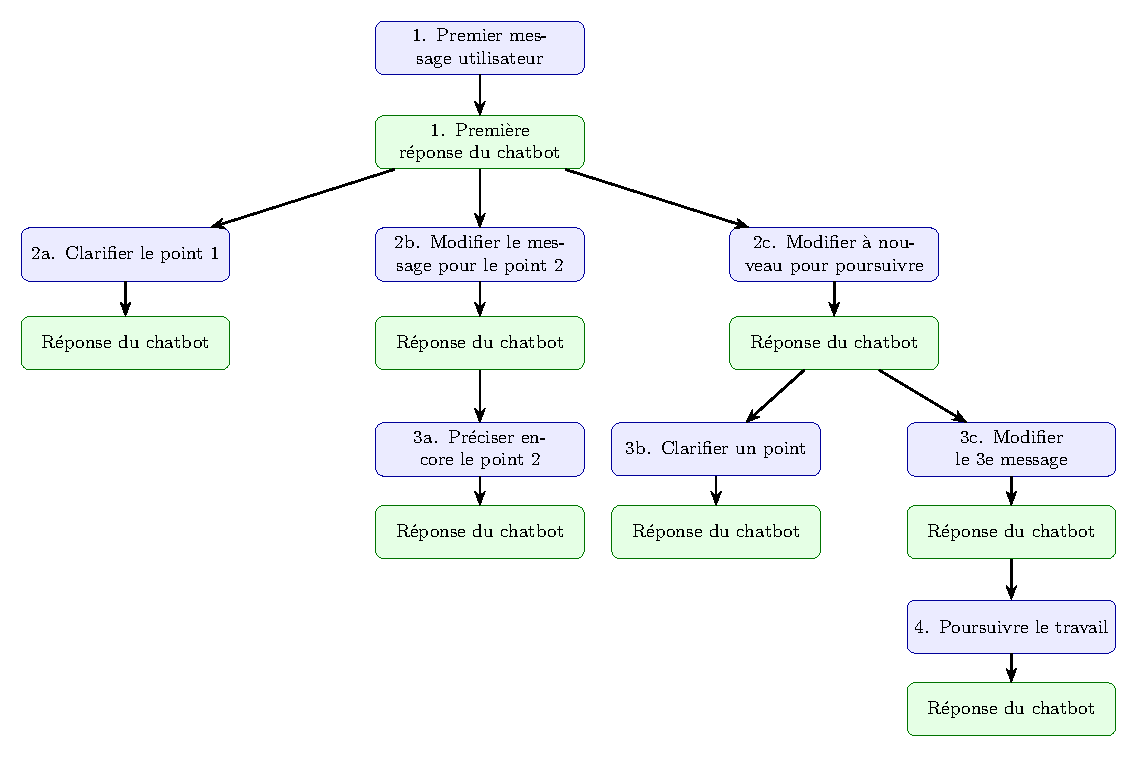
\includegraphics[width=\textwidth]{images/conv-branching-diagram.pdf}
\caption{Exemple d'arborescence des branches d'une conversation avec un chatbot.}
\label{fig}
\end{figure}

\subsubsection{Créer une nouvelle conversation pour chaque nouveau sujet}
Compte tenu de ce qui précède et de certains travaux \cite{Ruf_2025}, il est \textbf{plus efficace de créer une nouvelle conversation} pour aborder un sujet sans lien avec le précédent.

Deux options s'offrent à vous :
\begin{enumerate}
\def\labelenumi{\arabic{enumi}.}
\item
  \textbf{Créer une nouvelle conversation} dédiée au nouveau sujet.
\item
  \textbf{Modifier le premier message} de la conversation existante pour y introduire le nouveau sujet.
\end{enumerate}

Grâce à cette deuxième option, vous \textbf{réduisez le nombre de conversations} dans votre historique, ce qui permet de maintenir un \textbf{environnement propre et organisé}.

De même, vous pouvez \textbf{réutiliser la réponse d'un chatbot} en l'injectant dans une \textbf{nouvelle conversation} pour une tâche totalement différente, plutôt que de poursuivre dans la même discussion.
Cela permet, \textbf{une fois de plus, de limiter la taille du contexte}.

\subsubsection{Supprimer les conversations inutiles}
En réalité, lorsque vous envoyez un message à un chatbot, c'est toute la conversation qui est retransmise à chaque fois. Qui plus est, avant même vos messages, plusieurs éléments sont inclus : le \emph{prompt} du développeur, le \emph{prompt} système, des informations contextuelles (pays, heure, langue, navigateur, etc.), ainsi qu'un \textbf{résumé de chacune de vos conversations sauvegardées} \cite{mane2026context}. Ces résumés ajoutent du contexte au chatbot, mais ils ne sont pas toujours utiles. \textbf{N'hésitez pas à supprimer vos anciennes conversations si vous ne les utilisez plus.}

\subsubsection{Vider la mémoire à long terme}
Lorsque vous demandez à un chatbot de retenir une information au cours d'une conversation, celle-ci sera systématiquement incluse dans les nouvelles discussions. C'est ce qu'on appelle la \textbf{mémoire à long terme} \cite{openai2024memoire}. Pour l'optimiser, utilisez le menu dédié s'il existe, sinon créez une conversation dédiée dans laquelle vous demandez au chatbot de \textbf{lister les informations qu'il a mémorisées}, puis supprimez celles qui ne sont plus pertinentes.

\subsection{En tant qu'entreprise développant un agent}
\subsubsection{Prioriser les algorithmes à l'IA classique}
Dans de nombreux cas, de simples algorithmes de décision ou des IA de prédiction ou classification classiques sont suffisants.
Lorsque cela suffit, privilégiez l'utilisation de technologies moins complexes.

\subsubsection{Utiliser des petits modèles spécialisés.}
Nous avons vu plus tôt que le nombre de paramètres activés d'un modèle avait une grosse influence sur la consommation d'énergie pour le traitement d'un token.

Il faut prioriser l'utilisation de modèles petits et spécialisés. Certains développeurs ont mis à disposition sur Hugging Face des modèles qu'ils ont spécialisés sur une tâche à l'aide du fine-tuning. Il est mieux de récupérer des modèles déjà fine-tunés plutôt que de procéder à un fine-tuning à chaque fois.

Hugging Face : https://huggingface.co/

\subsubsection{Prompt engineering pour réduire le nombre de tokens en sortie}

De la même manière que l'utilisateur peut limiter les tokens en sortie, le développeur de l'application IA joue un rôle clé dans la taille des réponses générées.

Dans une application IA, le développeur intègre souvent un \emph{prompt système}, pris en compte par le LLM avant même la première requête de l'utilisateur. \textbf{Ce \emph{prompt système} doit préciser explicitement la forme attendue de la réponse}, afin de minimiser systématiquement le nombre de tokens en sortie.

\subsubsection{Context engineering pour réduire le nombre de tokens en entrée}
En tant que développeur, il est possible de concevoir des systèmes pour \textbf{réduire le contexte} en éliminant le bruit en ne conservant que les informations utiles.\\
Par exemple :
\begin{itemize}
\item
  Après une conversation de 10 messages, un LLM peut être sollicité pour \textbf{résumer ces échanges}. Ce résumé sera alors injecté dans les prochains messages, plutôt que l'intégralité des 10 messages initiaux.
\item
  Lors de l'utilisation de techniques comme le \textbf{RAG} (\emph{Retrieval-Augmented Generation}) ou la mémoire long terme, il est possible de \textbf{filtrer et sélectionner uniquement les éléments pertinents} du contexte.
\item
  \textbf{Lors d'un processus multi-étapes}, il est essentiel de \textbf{bien décomposer les étapes} pour ne fournir au LLM \textbf{que les informations strictement nécessaires à chaque étape}. Si besoin, les logs ou résultats intermédiaires peuvent être conservés dans le contexte pour les étapes suivantes.
\end{itemize}

Chaque développeur peut faire preuve de créativité pour \textbf{limiter le contexte envoyé au LLM}. Cela relève également du travail de l'ingénieur IA.

\subsubsection{Fine-tuning vs Few-shots-exemples}

Pour qu'un LLM produise une sortie correspondant aux attentes, plusieurs méthodes existent, comme l'ajout d'exemples ou le \emph{fine-tuning}. 
\textbf{Ajouter des exemples au contexte} (\emph{one-shot} ou \emph{few-shots}) est recommandé si l'agent ne sera pas utilisé de manière intensive. En revanche, pour une utilisation massive, il est préférable de réduire le nombre de tokens en entrée. Dans ce cas, le \emph{fine-tuning} permet au modèle de comprendre le type de réponse attendu \textbf{sans avoir besoin de lui fournir des exemples à chaque requête}. Cependant, le \emph{fine-tuning} a un \textbf{coût environnemental et financier élevé}. Il est donc recommandé uniquement si l'application sera utilisée à grande échelle.

\textbf{Comment décider entre \emph{few-shots} et \emph{fine-tuning} ?}
Pour déterminer le seuil à partir duquel le \emph{fine-tuning} devient plus rentable, il faut :

\begin{enumerate}
\def\labelenumi{\arabic{enumi}.}
\item
  Convertir en tokens la partie du \emph{prompt système} qui contient l'exemple du livrable.
\item
  Estimer le coût par requête en fonction de ce nombre de tokens.
\item
  Comparer ce coût cumulé au coût fixe du \emph{fine-tuning} (prédictible).
\end{enumerate}

Dès que le coût total des requêtes avec un \emph{prompt} long dépasse celui du \emph{fine-tuning}, il devient plus avantageux d'opter pour cette dernière méthode.

\subsubsection{Choisir un data center dans un pays à faible impact énergétique et hydrique}
Lorsqu'on décide d'héberger soi-même son modèle dans le cloud public, il est recommandé de sélectionner une région dotée d'un \textbf{bon score énergétique et hydrique} (faible facteur d'émission et PUE faible toute l'année). Dans la majorité des cas, les data centers du cloud public sont mieux optimisés à grande échelle que ceux des infrastructures privées.

Selon l'ADEME (2013), il est préférable, du point de vue des émissions carbone, d'héberger un modèle dans un pays à faible facteur d'émission, comme la Suède, la France ou la Suisse.

Les principaux fournisseurs de cloud indiquent la localisation de leurs data centers par région :

\begin{itemize}
\item
  Amazon Web Service :
  \href{https://aws.amazon.com/fr/about-aws/global-infrastructure/regions_az/}{\ul{https://aws.amazon.com/fr/about-aws/global-infrastructure/regions\_az/}}
\item
  Microsoft Azure :
  \href{https://learn.microsoft.com/en-us/azure/reliability/regions-list?tabs=all}{\ul{https://learn.microsoft.com/en-us/azure/reliability/regions-list?tabs=all}}
\item
  Google Cloud Platform :
  \href{https://datacenters.google/locations/}{\ul{https://datacenters.google/locations/}}
\item
  Salesforce :
  \href{https://help.salesforce.com/s/articleView?id=000396845&type=1}{\ul{https://help.salesforce.com/s/articleView?id=000396845\&type=1}}
\item
  OVH :
  \href{https://www.ovhcloud.com/en/datacenter/}{\ul{https://www.ovhcloud.com/en/datacenter/}}
\item
  Hostinger :
  \href{https://www.hostinger.com/support/1583267-where-are-hostinger-servers-located/}{\ul{https://www.hostinger.com/support/1583267-where-are-hostinger-servers-located/}}
\end{itemize}

Une fois la région du fournisseur de cloud pré-sélectionnée, il faut évaluer son PUE pour déterminer laquelle a la meilleure efficacité énergétique.

Vous pouvez retrouver les valeurs de PUE par région publiées par les principaux fournisseurs de cloud :

\begin{itemize}
\item
  \textbf{Amazon Web Services} :
  \href{https://sustainability.aboutamazon.com/products-services/aws-cloud}{\ul{https://sustainability.aboutamazon.com/products-services/aws-cloud}}
\item
  \textbf{Microsoft Azure} :
  \href{https://datacenters.microsoft.com/sustainability/efficiency/}{\ul{https://datacenters.microsoft.com/sustainability/efficiency/}}
\item
  \textbf{Google Cloud Platform} :
  \href{https://datacenters.google/efficiency/}{\ul{https://datacenters.google/efficiency/}}
\item
  \textbf{OVH} :
  \href{https://www.ovhcloud.com/sites/default/files/external_files/kpis_fy25.pdf}{\ul{https://www.ovhcloud.com/sites/default/files/external\_files/kpis\_fy25.pdf}}
\end{itemize}

Une fois une région à faible facteur d'émission et faible PUE sélectionnée, il faut vérifier qu'elle ne se trouve pas dans une région à risque de sécheresse.
Pour évaluer les risques liés à la disponibilité de l'eau, le \textbf{World Resources Institute (WRI)} propose une carte des régions à fort risque de sécheresse :\\
\href{https://www.wri.org/aqueduct/tools}{\ul{https://www.wri.org/aqueduct/tools}}.

Enfin, il faut regarder le WUE des data centers des fournisseurs. Bien qu'il ne soit pas toujours renseigné, il est possible de le récupérer sur le site des fournisseurs de cloud :

\begin{itemize}
\item
  \textbf{Amazon Web Services} :
  \href{https://sustainability.aboutamazon.com/products-services/aws-cloud/}
\item
  \textbf{Microsoft Azure} :
  \href{https://datacenters.microsoft.com/sustainability/efficiency/}
\item
  \textbf{Google Cloud Platform} : lien
  \href{https://services.google.com/fh/files/misc/measuring_the_environmental_impact_of_delivering_ai_at_google_scale.pdf}
\item
  \textbf{OVH} :
  \href{https://www.ovhcloud.com/sites/default/files/external_files/kpis_fy25.pdf}
\end{itemize}

\subsubsection{Moteur d'inférence}
Certains fournisseurs optimisent leurs modèles pour certains moteurs d'inférence \cite{nvidia2026llminference}. Le moteur adéquat est généralement renseigné dans le document de présentation du modèle.

\subsubsection{Utiliser le cache}

Dans certains cas, la fonctionnalité de \textbf{cache} permet de stocker et de réutiliser les calculs d'attention ainsi que les tokens d'un prompt déjà traité, évitant ainsi de tout recalculer à chaque requête.

\textbf{Cas d'usage optimisés avec le cache} :
\begin{itemize}
\item
  \textbf{Répétition d'un contexte volumineux} : par exemple lorsque vous envoyez fréquemment la même documentation dans le contexte, ou l'historique complet d'une conversation (cas d'un chatbot).
\item
  \textbf{Agents autonomes} : les agents effectuant des appels successifs en s'appuyant sur le même \textbf{prompt système} (instructions de base, outils disponibles, exemples de guidage) et un état partagé.
\item
  \textbf{Assistants de code} : analyse d'un dépôt de code volumineux et identique à chaque message.
\end{itemize}

Pour qu'un cache soit efficace, le préfixe du prompt (la partie à mettre en cache) doit être \textbf{strictement identique} d'une requête à l'autre. Le moindre espace ou caractère modifié au début du texte invalidera tout ou partie du cache existant.

\subsubsection{Traitement par lots (Batch processing)}
Le \textbf{batch processing} consiste à envoyer un grand nombre de requêtes à traiter simultanément. Cette méthode optimise l'inférence du LLM et permet de \textbf{réduire significativement} le coût énergétique et financier \cite{poddar2025sustainablenlpinsightsbenchmarking}.

En général, les fournisseurs de LLM via API proposent le \emph{batch processing} à \textbf{moitié prix} par rapport au traitement classique. Bien qu'il n'existe pas de données précises dans la littérature quantifiant cette réduction, on peut supposer que la variation du prix est corrélée à celle de l'impact énergétique.

Si vous n'avez pas besoin des réponses du LLM en temps réel et que vous avez un \textbf{volume important de requêtes quotidiennes}, il est préférable d'envoyer toutes les requêtes \textbf{en une seule fois}, par exemple à la fin de la journée.

\subsubsection{Modèles récents}
Il est essentiel de \textbf{rester informé} sur les nouveaux modèles, car certains peuvent offrir des performances équivalentes à celles de votre modèle actuel \textbf{tout en consommant significativement moins d'énergie}, grâce à une optimisation ou innovation.

\begin{figure}[htbp]
    \centering
    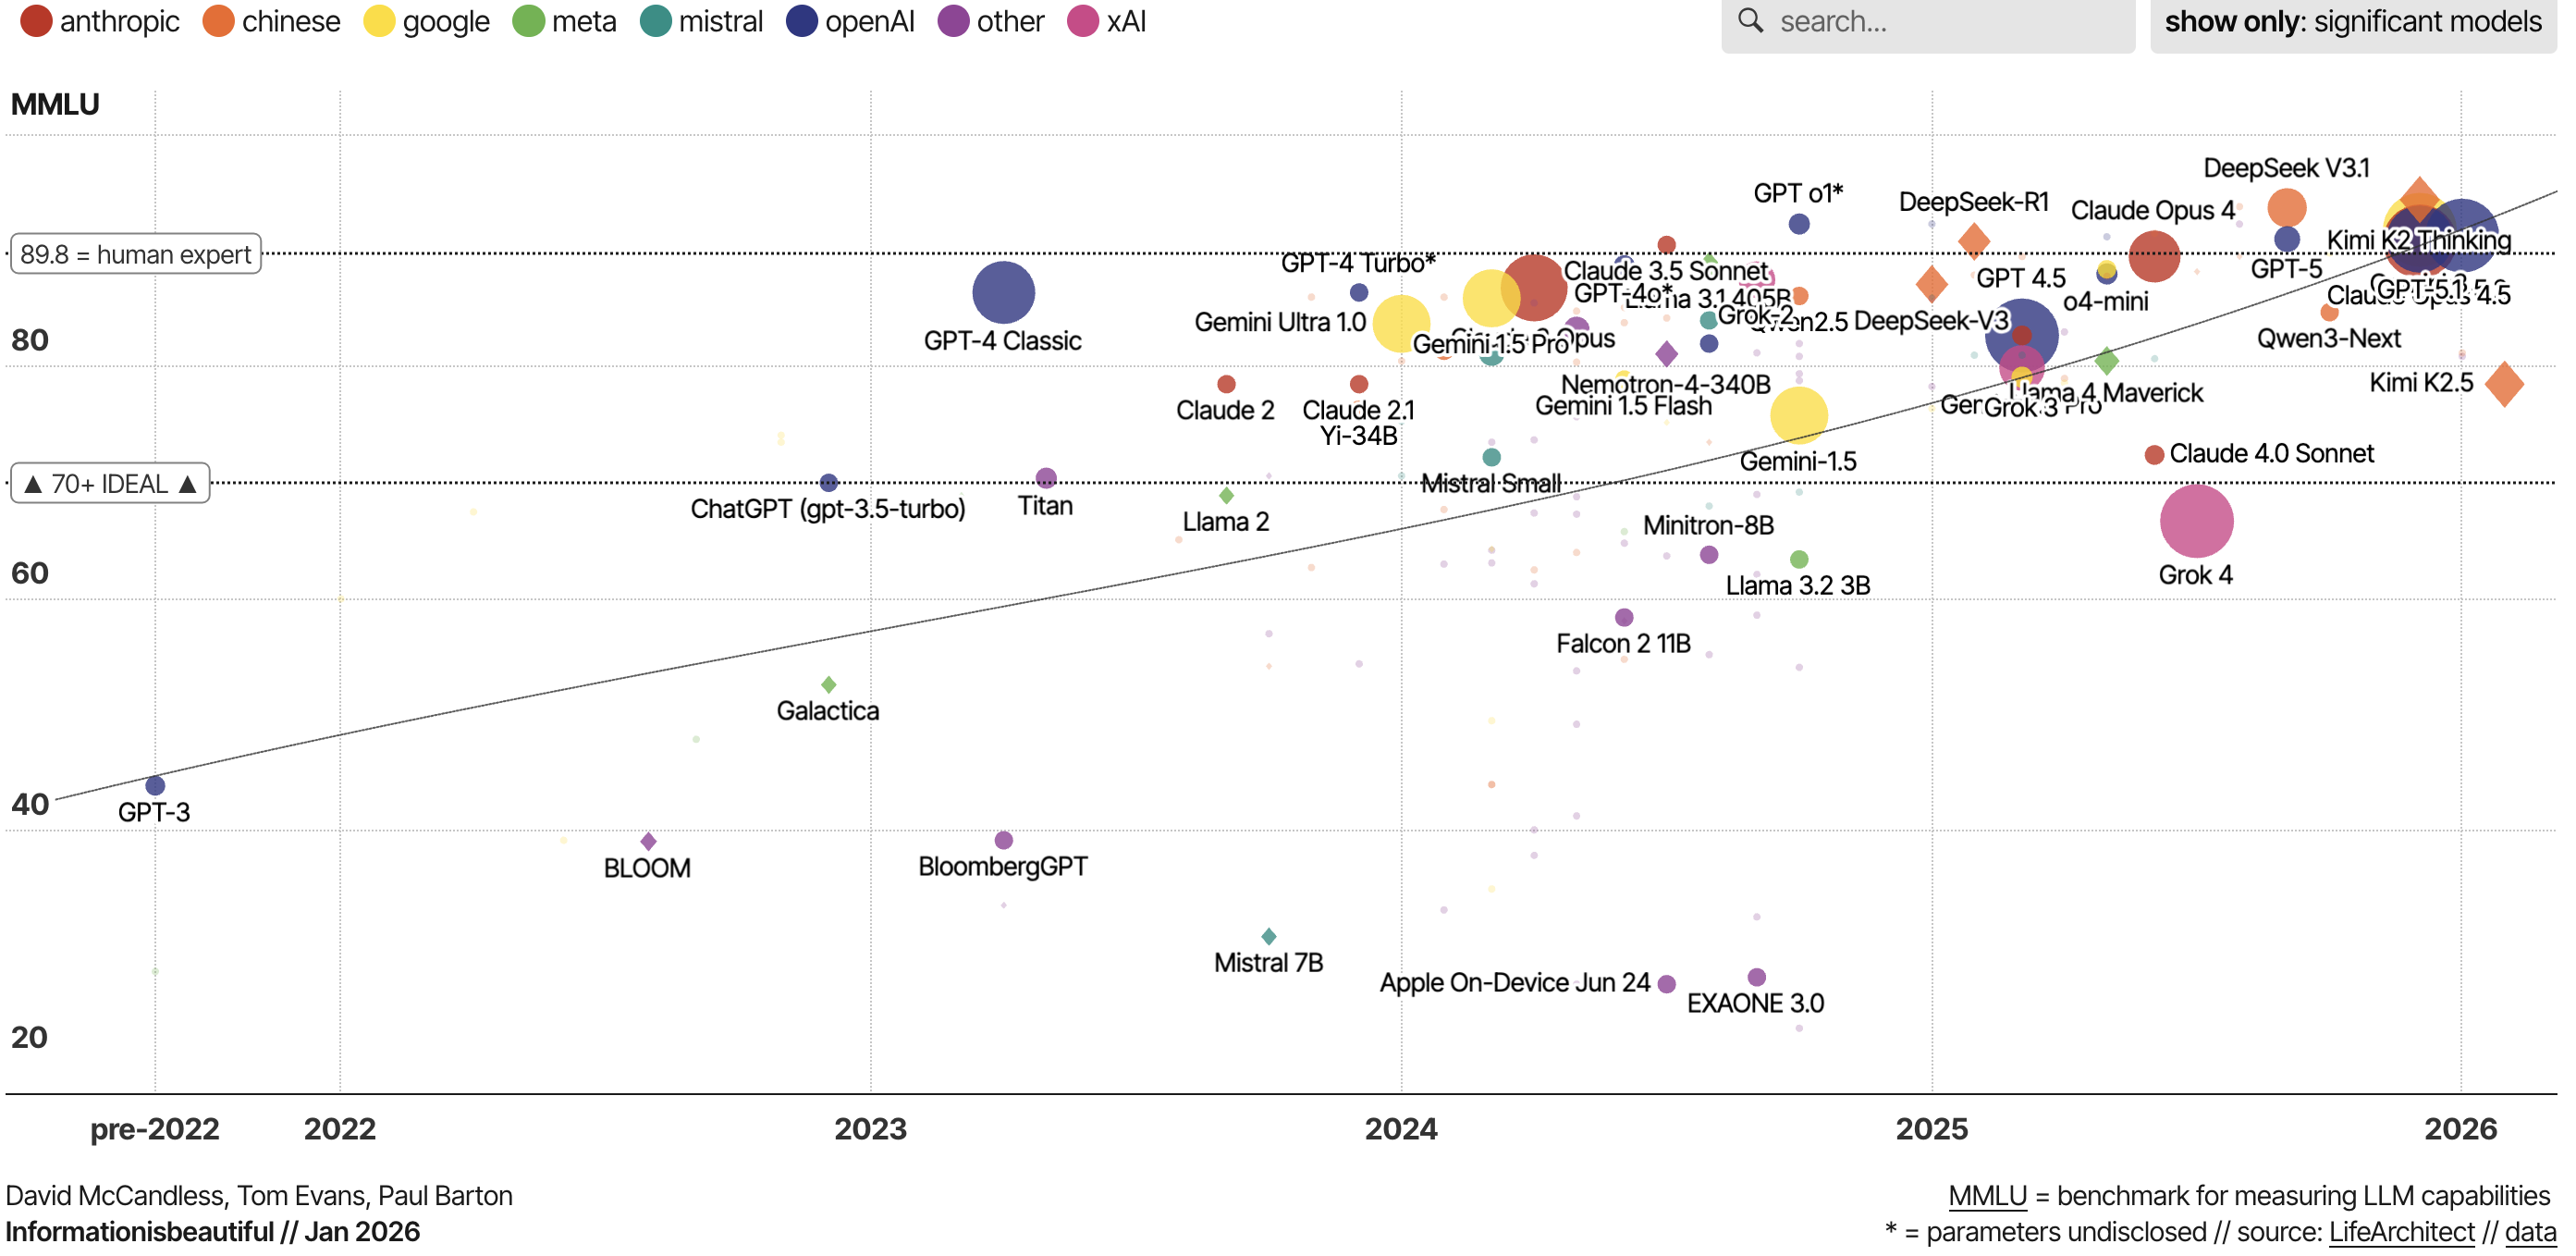
\includegraphics[width=0.8\textwidth]{images/Major-Large-Language-Models.png}
    \caption{Principaux LLM classés selon leurs capacités, en fonction du nombre de paramètres utilisés pour leur entraînement}
    \label{fig:architecture}
    
    \small
    \textit{Global landscape of LLMs and their performance. Reprinted under open access from David et al. \cite{david2025llm}}
\end{figure}

Pour la génération d'images par exemple, une étude suggère que les choix du type de modèle devraient tenir compte de la longueur prévue de la sortie : les modèles autorégressifs (les plus utilisés) restent préférables pour les réponses courtes (moins de 1024 tokens), tandis que les modèles de diffusion offrent des avantages indéniables pour les tâches de génération plus longues \cite{ruf2026diffusion}. 

Attention, changer de modèle peut induire une nouvelle phase de développement (tests, fine-tuning) impliquant un impact environnemental significatif.
